\documentclass{article}
\usepackage{amsmath}
\usepackage{amssymb}
\usepackage{tikz}
\usetikzlibrary{arrows.meta}

\begin{document}

\begin{figure}[h]
    \centering
    \begin{tikzpicture}[scale=1.5]
        % Define the nodes for the finite graph G_{k,n}
        \foreach \x in {0,...,9} {
            \node[circle, fill=yellow!80!black, inner sep=2pt] (A\x) at ({360/10*\x}:1) {};
        }
        
        % Draw edges for the finite graph G_{k,n}
        \draw[thick] (A0) -- (A1) -- (A2) -- (A3) -- (A4) -- (A5) -- (A6) -- (A7) -- (A8) -- (A9) -- cycle;
        \draw[thick] (A0) -- (A2);
        \draw[thick] (A1) -- (A3);
        \draw[thick] (A2) -- (A4);
        \draw[thick] (A3) -- (A5);
        \draw[thick] (A4) -- (A6);
        \draw[thick] (A5) -- (A7);
        \draw[thick] (A6) -- (A8);
        \draw[thick] (A7) -- (A9);
        \draw[thick] (A8) -- (A0);
        
        % Draw the dotted rectangle indicating the ball of radius r in graph-distance
        \draw[dotted, thick] (A0) -- (A2) -- (A4) -- (A6) -- (A8) -- (A0);
        
        % Draw the arrow indicating the isomorphism
        \draw[->, >=Stealth, thick] (A4) to[bend left=45] node[midway, above] {$\cong$} (A8);
        
        % Define the nodes for the infinite graph G_{k,\infty}
        \foreach \x in {0,...,19} {
            \node[circle, fill=red!80!black, inner sep=2pt] (B\x) at (\x*18:2) {};
        }
        
        % Draw the arrow indicating the isomorphism
        \draw[->, >=Stealth, thick] (A8) to[bend right=45] node[midway, below] {$\cong$} (B0);
        
        % Draw the line indicating the infinite graph G_{k,\infty}
        \draw[dotted, thick] (B0) -- (B19);
        
        % Label the infinite graph with Z
        \node at (20*18:2.5) {$\mathbb{Z}$};
        
        % Draw the label for the finite graph
        \node at (-1, -1) {\textbf{Illustration of the proof of Proposition \ref{pro: LWconv}: Any ball of radius $r < \lfloor n/2 \rfloor$ in graph-distance (indicated by the dotted rectangle) around any vertex in $G_{k,n}$ is isomorphic to the respective ball around $0$ in $G_{k,\infty}$. On the other hand, for given $r \geq 1$ we can choose $n \geq \lceil 2r \rceil$ so that each ball of radius $r$ in $G_{k,n}$ is isomorphic to the respective ball around $0$ in $G_{k,\infty}$.}};
    \end{tikzpicture}
    \caption{Illustration of the proof of Proposition \ref{pro: LWconv}: Any ball of radius $r < \lfloor n/2 \rfloor$ in graph-distance (indicated by the dotted rectangle) around any vertex in $G_{k,n}$ is isomorphic to the respective ball around $0$ in $G_{k,\infty}$. On the other hand, for given $r \geq 1$ we can choose $n \geq \lceil 2r \rceil$ so that each ball of radius $r$ in $G_{k,n}$ is isomorphic to the respective ball around $0$ in $G_{k,\infty}$.}
    \label{fig:proof_lwconv}
\end{figure}

\end{document}